\documentclass{standalone}
\usepackage{tikz}
\usepackage{ctex,siunitx}
\setCJKmainfont{Noto Serif CJK SC}
\usepackage{tkz-euclide}
\usepackage{amsmath}
\usetikzlibrary{patterns, calc,3d}
\usetikzlibrary {decorations.pathmorphing,decorations.pathreplacing,decorations.shapes}
\begin{document}
\small
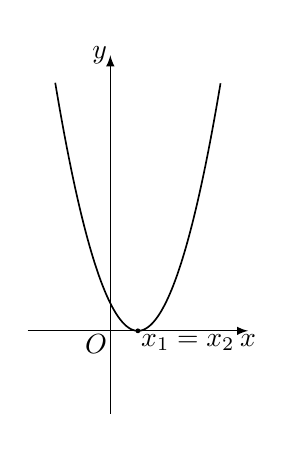
\begin{tikzpicture}[>=latex,scale=0.35,inner sep=1pt]
  \useasboundingbox(-3,-3.5)rectangle(5.5,11);
  \draw[->](-3,0)--(5,0)node[below]{$x$};
  \draw[->](0,-3)--(0,10)node[left]{$y$};
  \draw[samples=200,domain=-2:4,semithick]plot({\x},{\x*\x-2*\x+1});
  \node at (0,0)[below left]{$O$};
  \fill (1,0)circle(2.5pt)node[below right]{$x_1=x_2$};
\end{tikzpicture}
\end{document}